\documentclass{article}
\usepackage{tikz}
\usepackage{lipsum} % for generating dummy text
\usepackage{xparse}
\usepackage{amsmath}
\usepackage{amsfonts}
\usepackage{placeins}


% Define a new command for drawing the ellipse
\NewDocumentCommand{\drawellipse}{m m m m m o}{
    \def\centerX{#1}
    \def\centerY{#2}
    \def\widthR{#3}
    \def\heightR{#4}
    \def\angle{#5}
    
    \draw (\centerX,\centerY) ellipse [x radius=\widthR, y radius=\heightR];
    \fill ({\centerX + \widthR*cos(\angle)},{\centerY + \heightR*sin(\angle)}) circle [radius=0.075];
    
    % If target node is provided, use it, otherwise fall back to default behavior
    \IfNoValueTF{#6}{
        \draw ({\centerX + \widthR*cos(\angle)},{\centerY + \heightR*sin(\angle)}) -- ({\centerX + .5 + \widthR*cos(\angle)}, {\centerY + \heightR*sin(\angle)});
    }{
        \draw ({\centerX + \widthR*cos(\angle)},{\centerY + \heightR*sin(\angle)}) -- (#6);
    }
}

\NewDocumentCommand{\drawellipseX}{m m m m m}{
    \def\centerX{#1}
    \def\centerY{#2}
    \def\widthR{#3}
    \def\heightR{#4}
    \def\angle{#5}
    
    \draw (\centerX,\centerY) ellipse [x radius=\widthR, y radius=\heightR];
    \fill ({\centerX + \widthR*cos(\angle)},{\centerY + \heightR*sin(\angle)}) circle [radius=0.075];


    \draw ({\centerX + \widthR*cos(\angle)},{\centerY + \heightR*sin(\angle)}) -- ({\centerX + .5 + \widthR*cos(\angle)}, {\centerY + + \heightR*sin(\angle)});
    
     \draw ({\centerX + \widthR*cos(\angle)},{\centerY + \heightR*sin(\angle)}) -- ({\centerX + .5 + \widthR*cos(\angle)}, {\centerY + .2 + \heightR*sin(\angle)});

}


% Define a new command for the graph
\newcommand{\drawgraph}[2]{
    % Nodes
    \node[circle, draw, minimum size=0.5cm] (f{#1#2}) at (#1,#2+1) {f};
    \node[circle, draw, minimum size=0.5cm] (v{#1#2}) at (#1,#2) {v};
    \node[circle, draw, minimum size=0.5cm] (x{#1#2}) at (#1,#2-1) {x};
    
    % Edges
    \draw[->] (x{#1#2}) -- (v{#1#2});
    \draw[->] (v{#1#2}) -- (f{#1#2});
}


\begin{document}

\section{Notation and Nomenclature}


\section{Pseudo-linear form}

Derivation of Peyman Milanfar's gradient
\begin{align*}
\mathrm{d}[\mathbf{f}(\mathbf{x})] & =\mathrm{d}[\mathbf{A}(\mathbf{x}) \mathbf{x}] \\
& =\mathrm{d}[\mathbf{A}(\mathbf{x})] \mathbf{x}+\mathbf{A}(\mathbf{x}) \mathrm{d} \mathbf{x} \\
& =\operatorname{vec}\{\mathrm{d}[\mathbf{A}(\mathbf{x})] \mathbf{x}\}+\mathbf{A}(\mathbf{x}) \mathrm{d} \mathbf{x} \\
& =\operatorname{vec}\{\mathbf{I} \mathrm{d}[\mathbf{A}(\mathbf{x})] \mathbf{x}\}+\mathbf{A}(\mathbf{x}) \mathrm{d} \mathbf{x} \\
& =\left(\mathbf{x}^T \otimes \mathbf{I}\right) \operatorname{vec}\{\mathrm{d}[\mathbf{A}(\mathbf{x})]\}+\mathbf{A}(\mathbf{x}) \mathrm{d} \mathbf{x} \\
& =\left(\mathbf{x}^T \otimes \mathbf{I}\right) \mathrm{D} \operatorname{vec}[\mathbf{A}(\mathbf{x})] \mathrm{d} \mathbf{x}+\mathbf{A}(\mathbf{x}) \mathrm{d} \mathbf{x} \\
& =\left[\left(\mathbf{x}^T \otimes \mathbf{I}\right) \mathrm{D} \operatorname{vec}[\mathbf{A}(\mathbf{x})]+\mathbf{A}(\mathbf{x})\right] \mathrm{d} \mathbf{x}
\end{align*}

\begin{figure}[h]
    \centering
    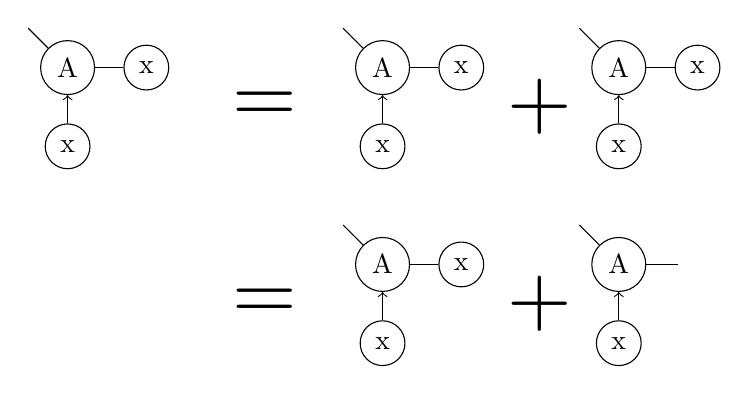
\begin{tikzpicture}
        \def\x{0}
        \def\y{0}
        \node[circle, draw, minimum size=0.5cm] (A) at (\x,\y+1) {A};
        \node[circle, draw, minimum size=0.5cm] (x) at (\x,\y) {x};
        \draw[->] (x) -- (A);
        \node[circle, draw, minimum size=0.5cm] (x2) at (\x+1,\y+1) {x};
        \draw (A) -- (x2);
        \draw (A) -- (\x-.5,\y+1.5);
        \drawellipse{\x+.5}{\y+.5}{1.25}{1.25}{180/4}
        
        % Equals sign
        \node[scale=3] at (2.5,\y+.5) {=};

        \def\x{4}
        \node[circle, draw, minimum size=0.5cm] (A) at (\x,\y+1) {A};
        \node[circle, draw, minimum size=0.5cm] (x) at (\x,\y) {x};
        \draw[->] (x) -- (A);
        \node[circle, draw, minimum size=0.5cm] (x2) at (\x+1,\y+1) {x};
        \draw (A) -- (x2);
        \draw (A) -- (\x-.5,\y+1.5);
        \drawellipse{\x}{\y+.5}{.6}{1.1}{180/3}
        
        % Plus sign
        \node[scale=3] at (\x+2,\y+.5) {+};
        
        \def\x{7}
        \node[circle, draw, minimum size=0.5cm] (A) at (\x,\y+1) {A};
        \node[circle, draw, minimum size=0.5cm] (x) at (\x,\y) {x};
        \draw[->] (x) -- (A);
        \node[circle, draw, minimum size=0.5cm] (x2) at (\x+1,\y+1) {x};
        \draw (A) -- (x2);
        \draw (A) -- (\x-.5,\y+1.5);
        \drawellipse{\x+1}{\y+1}{.4}{.4}{180/3}

        % Equals sign
        \def\x{0}
        \def\y{-2.5}
        \node[scale=3] at (2.5,\y+.5) {=};

        \def\x{4}
        \node[circle, draw, minimum size=0.5cm] (A) at (\x,\y+1) {A};
        \node[circle, draw, minimum size=0.5cm] (x) at (\x,\y) {x};
        \draw[->] (x) -- (A);
        \node[circle, draw, minimum size=0.5cm] (x2) at (\x+1,\y+1) {x};
        \draw (A) -- (x2);
        \draw (A) -- (\x-.5,\y+1.5);
        \drawellipse{\x}{\y+1}{.5}{.5}{180/3}
        
        % Plus sign
        \node[scale=3] at (\x+2,\y+.5) {+};
        
        \def\x{7}
        \node[circle, draw, minimum size=0.5cm] (A) at (\x,\y+1) {A};
        \node[circle, draw, minimum size=0.5cm] (x) at (\x,\y) {x};
        \draw[->] (x) -- (A);
        \draw (A) -- (\x+.75,\y+1);
        \draw (A) -- (\x-.5,\y+1.5);
    \end{tikzpicture}
    \caption{Visualization of pseudo-linear gradient.}
\end{figure}

Note, a third way to derive the gradient is to use index notation:
\begin{align*}
f_i(\mathbf{x}) &= A_{ij}(\mathbf{x}) x_j \\
\Rightarrow \mathrm{d} f_i &= \frac{\partial f_i}{\partial x_k} \mathrm{d} x_k \\
&= \left( \frac{\partial A_{ij}}{\partial x_k} x_j + A_{ij} \delta_{jk} \right) \mathrm{d} x_k \\
&= \left( \frac{\partial A_{ij}}{\partial x_k} x_j + A_{ik} \right) \mathrm{d} x_k \\
\end{align*}


\section{Chain Rule}

Standard chain rule.
Here we let $f\in\mathbb R^d\to \mathbb R$ be a scalar function, and $v\in\mathbb R^d\to \mathbb R^d$ be a vector function as used in backprop.

\begin{figure}[h]
    \centering
    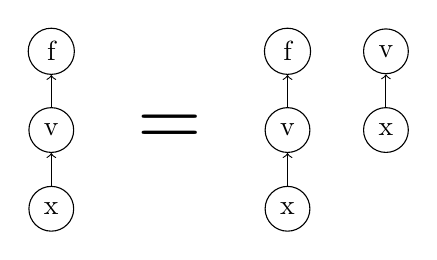
\begin{tikzpicture}
        \drawgraph{0}{0}
        \drawellipse{0}{0}{.75}{1.5}{180/4}
        % Equals sign
        \node[scale=3] at (1.5,0) {=};
        \drawgraph{3}{0}

        \def\loc{4.25}
        \node[circle, draw, minimum size=0.5cm] (v) at (\loc,1) {v};
        \node[circle, draw, minimum size=0.5cm] (x) at (\loc,0) {x};
        \draw[->] (x) -- (v);

        \drawellipse{3}{1}{.5}{.5}{0}[v]
        
        \drawellipse{\loc}{1}{.5}{.5}{0}

    \end{tikzpicture}
    \caption{Visualization of the Chain Rule: $J_{f\circ v}(x) = \nabla_{\!f}(v(x)) J_v(x)$.}
\end{figure}

% You can add more content or dummy text
% \lipsum[1] % generates some random text
\section{Computation of the Hessian}

Derivation of Yaroslav Bulatov's chain rule for the Hessian.
See Figure~\ref{fig:hessian}.

In index notation, the Hessian of $f(v(x))$ is
\[
H_{ij}(x) = \sum_{k=1}^d \sum_{l=1}^d \frac{\partial^2 f}{\partial u_k \partial u_l}(v(x)) \frac{\partial v_k}{\partial x_i}(x) \frac{\partial v_l}{\partial x_j}(x) + \frac{\partial f}{\partial u_k}(v(x)) \frac{\partial^2 v_k}{\partial x_i \partial x_j}(x)
.
\]
In matrix notation it is
\[
H(x) = Dv(x)^T \cdot D^2f(v(x)) \cdot Dv(x) + \sum_{k=1}^d \frac{\partial f}{\partial u_k}(v(x)) \frac{\partial^2 v_k}{\partial x \partial x^T}(x).
\]
Neither of them are terribly legible.

% https://cs.stackexchange.com/questions/146526/finding-the-cost-of-hessian-vector-product-computation
% or https://community.wolfram.com/groups/-/m/t/2437093

\begin{figure}[h]
    \centering
    \begin{tikzpicture}
        % Step 1: Initial function with two ellipses
        \drawgraph{0}{0}
        \drawellipse{0}{0}{1}{1.8}{180/4}
        \drawellipse{0}{0}{.75}{1.5}{180/4}
        
        % Equals sign for step 2
        \node[scale=3] at (2,0) {=};
        
        % Step 2: Apply the chain rule 
        \drawgraph{4}{0}
        \node[circle, draw, minimum size=0.5cm] (va) at (5.25,1) {v};
        \node[circle, draw, minimum size=0.5cm] (xa) at (5.25,0) {x};
        \draw[->] (xa) -- (va);
        \drawellipse{4}{1}{.4}{.4}{0}[va]
        \drawellipse{4.6}{.1}{1.4}{2}{180/3.5}
        \drawellipse{5.25}{1}{.4}{.4}{0}
        
        % Equals sign for step 2
        \def\y{-4.5}
        \node[scale=3] at (2,\y) {=};
 
        % Step 3: Apply the product rule of differentiation
        \def\x{4}
        \drawgraph{\x}{\y}
        \node[circle, draw, minimum size=0.5cm] (vb) at (\x+1.25,\y+1) {v};
        \node[circle, draw, minimum size=0.5cm] (xb) at (\x+1.25,\y) {x};
        \draw[->] (xb) -- (vb);
        \drawellipse{\x}{\y+1}{.4}{.4}{0}[vb]
        \drawellipse{\x}{\y}{.85}{1.9}{180/3.5}
        \drawellipse{\x+1.25}{\y+1}{.4}{.4}{0}
        
        % Plus sign
        \node[scale=3] at (6.25,\y) {+};

        % Second term of product rule
        \def\x{7.5}
        \drawgraph{\x}{\y}
        \node[circle, draw, minimum size=0.5cm] (vc) at (\x+1.25,\y+1) {v};
        \node[circle, draw, minimum size=0.5cm] (xc) at (\x+1.25,\y) {x};
        \draw[->] (xc) -- (vc);
        \drawellipse{\x}{\y+1}{.4}{.4}{0}[vc]
        \drawellipse{\x+1.25}{\y+.5}{.6}{1.2}{180/3.5}
        \drawellipse{\x+1.25}{\y+1}{.4}{.4}{0}
        
        % Third equals sign
        \def\y{-9}
        \node[scale=3] at (2,\y) {=};
        
        \def\x{4}
        \drawgraph{\x}{\y}
        \node[circle, draw, minimum size=0.5cm] (vb) at (\x+1.25,\y+1) {v};
        \node[circle, draw, minimum size=0.5cm] (xb) at (\x+1.25,\y) {x};
        \draw[->] (xb) -- (vb);
        \node[circle, draw, minimum size=0.5cm] (vb2) at (\x+2.5,\y+1.5) {v};
        \node[circle, draw, minimum size=0.5cm] (xb2) at (\x+2.5,\y+.5) {x};
        \draw[->] (xb2) -- (vb2);
        \drawellipse{\x}{\y+1}{.4}{.4}{0}[vb]
        \drawellipse{\x}{\y+1}{.5}{.5}{180/2}[vb2]
        \drawellipse{\x+1.25}{\y+1}{.4}{.4}{0}
        \drawellipse{\x+2.5}{\y+1.5}{.4}{.4}{0}
        
        % Plus sign
        \node[scale=3] at (7.5,\y) {+};

        \def\x{8.5}
        \drawgraph{\x}{\y}
        \node[circle, draw, minimum size=0.5cm] (vc) at (\x+1.25,\y+1) {v};
        \node[circle, draw, minimum size=0.5cm] (xc) at (\x+1.25,\y) {x};
        \draw[->] (xc) -- (vc);
        \drawellipse{\x}{\y+1}{.4}{.4}{0}[vc]
        \drawellipse{\x+1.25}{\y+1}{.4}{.4}{0}
        \drawellipse{\x+1.25}{\y+1}{.5}{.5}{180/4}

        
    \end{tikzpicture}
    \caption{Visualization of the Computation of the Hessian: \(
H_{f\circ v}(x) = Dv(x)^T \cdot D^2f(v(x)) \cdot Dv(x) + \sum_{k=1}^d \frac{\partial f}{\partial u_k}(v(x)) \frac{\partial^2 v_k}{\partial x \partial x^T}(x).
\).}
    \label{fig:hessian}
\end{figure}

\section{Quadratic form}
A common gradient from statistics, is the least squares $\nabla_x \|A x-b\|_2^2 = \nabla_x (Ax)^T(Ax) - 2b^TAx + b^Tb $.
See Figure~\ref{fig:quadratic}.

\begin{figure}[h!]\label{fig:quadratic}
    \centering
    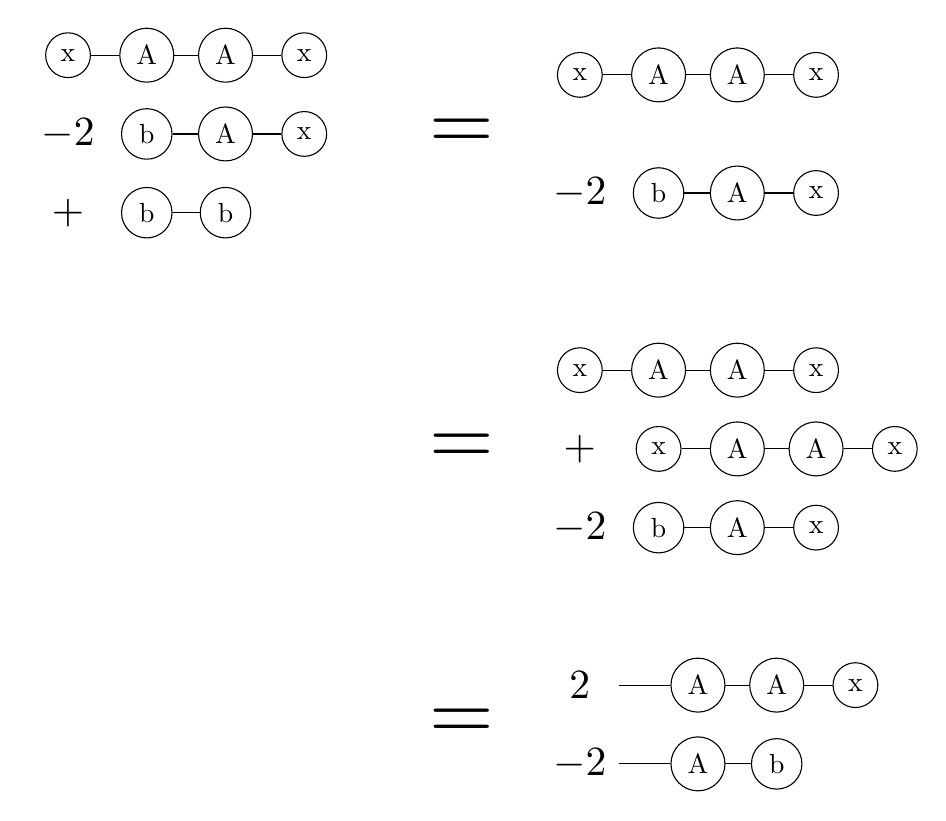
\begin{tikzpicture}
        \def\x{0}
        \def\y{0}
        \node[circle, draw, minimum size=0.5cm] (x1) at (\x,\y) {x};
        \node[circle, draw, minimum size=0.5cm] (A1) at (\x+1,\y) {A};
        \node[circle, draw, minimum size=0.5cm] (A2) at (\x+2,\y) {A};
        \node[circle, draw, minimum size=0.5cm] (x2) at (\x+3,\y) {x};
        \draw (x1) -- (A1) -- (A2) -- (x2);
        
        \node[scale=1.5] at (\x,\y-1) {$-2$};
        \node[circle, draw, minimum size=0.5cm] (b1) at (\x+1,\y-1) {b};
        \node[circle, draw, minimum size=0.5cm] (A3) at (\x+2,\y-1) {A};
        \node[circle, draw, minimum size=0.5cm] (x3) at (\x+3,\y-1) {x};
        \draw (b1) -- (A3) -- (x3);

        \node[scale=1.5] at (\x,\y-2) {+};
        \node[circle, draw, minimum size=0.5cm] (b2) at (\x+1,\y-2) {b};
        \node[circle, draw, minimum size=0.5cm] (b3) at (\x+2,\y-2) {b};
        \draw (b2) -- (b3);

        \drawellipse{\x+1.5}{\y-1}{2.5}{2}{180/4}

        \node[scale=3] at (\x+5,\y-1) {=};
        
        \def\x{6.5}
        \def\y{-.25}
        \node[circle, draw, minimum size=0.5cm] (x1) at (\x,\y) {x};
        \node[circle, draw, minimum size=0.5cm] (A1) at (\x+1,\y) {A};
        \node[circle, draw, minimum size=0.5cm] (A2) at (\x+2,\y) {A};
        \node[circle, draw, minimum size=0.5cm] (x2) at (\x+3,\y) {x};
        \draw (x1) -- (A1) -- (A2) -- (x2);
        \drawellipse{\x+1.5}{\y}{2.1}{.65}{180/4}
        
        \def\y{-.75}
        \node[scale=1.5] at (\x,\y-1) {$-2$};
        \node[circle, draw, minimum size=0.5cm] (b1) at (\x+1,\y-1) {b};
        \node[circle, draw, minimum size=0.5cm] (A3) at (\x+2,\y-1) {A};
        \node[circle, draw, minimum size=0.5cm] (x3) at (\x+3,\y-1) {x};
        \draw (b1) -- (A3) -- (x3);
        \drawellipse{\x+1.5}{\y-1}{2.1}{.65}{180/4}

        \def\y{-4}
        \node[scale=3] at (\x-1.5,\y-1) {=};
        
        \node[circle, draw, minimum size=0.5cm] (x1) at (\x,\y) {x};
        \node[circle, draw, minimum size=0.5cm] (A1) at (\x+1,\y) {A};
        \node[circle, draw, minimum size=0.5cm] (A2) at (\x+2,\y) {A};
        \node[circle, draw, minimum size=0.5cm] (x2) at (\x+3,\y) {x};
        \draw (x1) -- (A1) -- (A2) -- (x2);
        \drawellipse{\x}{\y}{.4}{.4}{180/2}

        \def\y{-5}
        \node[scale=1.5] at (\x,\y) {+};
        \def\x{7.5}
        
        \node[circle, draw, minimum size=0.5cm] (x1) at (\x,\y) {x};
        \node[circle, draw, minimum size=0.5cm] (A1) at (\x+1,\y) {A};
        \node[circle, draw, minimum size=0.5cm] (A2) at (\x+2,\y) {A};
        \node[circle, draw, minimum size=0.5cm] (x2) at (\x+3,\y) {x};
        \draw (x1) -- (A1) -- (A2) -- (x2);
        \drawellipse{\x+3}{\y}{.4}{.4}{180/2}

        \def\x{6.5}
        \node[scale=1.5] at (\x,\y-1) {$-2$};
        \node[circle, draw, minimum size=0.5cm] (b1) at (\x+1,\y-1) {b};
        \node[circle, draw, minimum size=0.5cm] (A3) at (\x+2,\y-1) {A};
        \node[circle, draw, minimum size=0.5cm] (x3) at (\x+3,\y-1) {x};
        \draw (b1) -- (A3) -- (x3);
        \drawellipse{\x+3}{\y-1}{.4}{.4}{180/4}

        \def\y{-8}
        \node[scale=3] at (\x-1.5,\y-.5) {=};
        \node[scale=1.5] at (\x,\y) {2};
        \node[scale=1.5] at (\x,\y-1) {$-2$};
        \def\x{7}

        \node[circle, draw, minimum size=0.5cm] (A1) at (\x+1,\y) {A};
        \node[circle, draw, minimum size=0.5cm] (A2) at (\x+2,\y) {A};
        \node[circle, draw, minimum size=0.5cm] (x3) at (\x+3,\y) {x};
        \draw (\x,\y) -- (A1) -- (A2) -- (x3);

        \node[circle, draw, minimum size=0.5cm] (A3) at (\x+1,\y-1) {A};
        \node[circle, draw, minimum size=0.5cm] (b1) at (\x+2,\y-1) {b};
        \draw (\x,\y-1) -- (A3) -- (b1);
        
    \end{tikzpicture}
    \caption{Least squares gradient, $\nabla_x \|A x-b\|_2^2 = 2 A^TAx - 2Ab$.}
\end{figure}

Once the gradient has been derived, we can solve for $x$ to get the usual solution $x=(A^TA)^{-1}Ab$.

\section{Quadratic form 2}
In machine learning we sometimes want a ``matrix shaped'' gradient that we can easily add to the original matrix for gradient descent.
Let's define a derivative notation with two edges going out for this purpose.
Then we can derive the gradient with respect to $X$ of
$\nabla_X \|X a-b\|_2^2$.
See Figure~\ref{fig:quadratic2}.



\begin{figure}[h]\label{fig:quadratic2}
    \centering
    \begin{tikzpicture}
        \def\x{0}
        \def\y{0}
        \node[circle, draw, minimum size=0.5cm] (a1) at (\x,\y) {a};
        \node[circle, draw, minimum size=0.5cm] (X1) at (\x+1,\y) {X};
        \node[circle, draw, minimum size=0.5cm] (X2) at (\x+2,\y) {X};
        \node[circle, draw, minimum size=0.5cm] (a2) at (\x+3,\y) {a};
        \draw (a1) -- (X1) -- (X2) -- (a2);
        
        \node[scale=1.5] at (\x,\y-1) {$-2$};
        \node[circle, draw, minimum size=0.5cm] (b1) at (\x+1,\y-1) {b};
        \node[circle, draw, minimum size=0.5cm] (X3) at (\x+2,\y-1) {X};
        \node[circle, draw, minimum size=0.5cm] (a3) at (\x+3,\y-1) {a};
        \draw (b1) -- (X3) -- (a3);

        \node[scale=1.5] at (\x,\y-2) {+};
        \node[circle, draw, minimum size=0.5cm] (b2) at (\x+1,\y-2) {b};
        \node[circle, draw, minimum size=0.5cm] (b3) at (\x+2,\y-2) {b};
        \draw (b2) -- (b3);

        \drawellipseX{\x+1.5}{\y-1}{2.5}{2}{180/4}

        \node[scale=3] at (\x+5,\y-1) {=};
        
        \def\x{6.5}
        \def\y{-.25}
        \node[circle, draw, minimum size=0.5cm] (a1) at (\x,\y) {a};
        \node[circle, draw, minimum size=0.5cm] (X1) at (\x+1,\y) {X};
        \node[circle, draw, minimum size=0.5cm] (X2) at (\x+2,\y) {X};
        \node[circle, draw, minimum size=0.5cm] (a2) at (\x+3,\y) {a};
        \draw (a1) -- (X1) -- (X2) -- (a2);
        \drawellipseX{\x+1.5}{\y}{2.1}{.65}{180/4}
        
        \def\y{-.75}
        \node[scale=1.5] at (\x,\y-1) {$-2$};
        \node[circle, draw, minimum size=0.5cm] (b1) at (\x+1,\y-1) {b};
        \node[circle, draw, minimum size=0.5cm] (X3) at (\x+2,\y-1) {X};
        \node[circle, draw, minimum size=0.5cm] (a3) at (\x+3,\y-1) {a};
        \draw (b1) -- (X3) -- (a3);
        \drawellipseX{\x+1.5}{\y-1}{2.1}{.65}{180/4}

        \def\y{-4}
        \node[scale=3] at (\x-1.5,\y-1) {=};
        
        \node[circle, draw, minimum size=0.5cm] (x1) at (\x,\y) {a};
        \node[circle, draw, minimum size=0.5cm] (A1) at (\x+1,\y) {X};
        \node[circle, draw, minimum size=0.5cm] (A2) at (\x+2,\y) {X};
        \node[circle, draw, minimum size=0.5cm] (x2) at (\x+3,\y) {a};
        \draw (x1) -- (A1) -- (A2) -- (x2);
        \drawellipseX{\x+1}{\y}{.4}{.4}{180/2}

        \def\y{-5}
        \node[scale=1.5] at (\x,\y) {+};
        \def\x{7.5}
        
        \node[circle, draw, minimum size=0.5cm] (x1) at (\x,\y) {a};
        \node[circle, draw, minimum size=0.5cm] (A1) at (\x+1,\y) {X};
        \node[circle, draw, minimum size=0.5cm] (A2) at (\x+2,\y) {X};
        \node[circle, draw, minimum size=0.5cm] (x2) at (\x+3,\y) {a};
        \draw (x1) -- (A1) -- (A2) -- (x2);
        \drawellipseX{\x+2}{\y}{.4}{.4}{180/2}

        \def\x{6.5}
        \node[scale=1.5] at (\x,\y-1) {$-2$};
        \node[circle, draw, minimum size=0.5cm] (b1) at (\x+1,\y-1) {b};
        \node[circle, draw, minimum size=0.5cm] (A3) at (\x+2,\y-1) {X};
        \node[circle, draw, minimum size=0.5cm] (x3) at (\x+3,\y-1) {a};
        \draw (b1) -- (A3) -- (x3);
        \drawellipseX{\x+2}{\y-1}{.4}{.4}{180/4}

        \def\y{-8}
        \node[scale=3] at (\x-1.5,\y-.5) {=};
        \node[scale=1.5] at (\x,\y) {2};
        \node[scale=1.5] at (\x,\y-1) {$-2$};
        
        \def\x{7.25}
        \node[circle, draw, minimum size=0.5cm] (a1) at (\x,\y) {a};
        \node[circle, draw, minimum size=0.5cm] (A2) at (\x+2,\y) {X};
        \node[circle, draw, minimum size=0.5cm] (x3) at (\x+3,\y) {a};
        \draw (a1) -- (\x+.9,\y) -- (\x+1.1,\y-.4);
        \draw (\x+.9,\y+.4) -- (\x+1.1,\y) -- (A2) -- (x3);

        \node[circle, draw, minimum size=0.5cm] (a1) at (\x,\y-1) {a};
        \node[circle, draw, minimum size=0.5cm] (b1) at (\x+2,\y-1) {b};
        \draw (a1) -- (\x+.9,\y-1) -- (\x+1.1,\y-.4-1);
        \draw (\x+.9,\y+.4-1) -- (\x+1.1,\y-1) -- (b1);


        \def\y{-11}
        \def\x{6.5}
        \node[scale=3] at (\x-1.5,\y-.5) {=};
        \node[scale=1.5] at (\x,\y) {2};
        \node[scale=1.5] at (\x,\y-1) {$-2$};
        
        \def\x{7.25}
        \node[circle, draw, minimum size=0.5cm] (a1) at (\x,\y) {a};
        \node[circle, draw, minimum size=0.5cm] (A2) at (\x+2,\y) {X};
        \node[circle, draw, minimum size=0.5cm] (x3) at (\x+3,\y) {a};
        \draw (a1) -- (\x+.5,\y);
        \draw (\x+2-.6, \y) -- (A2) -- (x3);

        \node[circle, draw, minimum size=0.5cm] (a1) at (\x,\y-1) {a};
        \node[circle, draw, minimum size=0.5cm] (b1) at (\x+2,\y-1) {b};
        \draw (a1) -- (\x+.5,\y-1);
        \draw (\x+2-.5,\y-1) -- (b1);


        \def\y{-14}
        \def\x{6.5}
        \node[scale=3] at (\x-1.5,\y) {=};
        \node[scale=1.5] at (\x,\y) {2};
        
        \def\x{7.25}
        \node[circle, draw, minimum size=0.5cm] (a1) at (\x,\y) {a};
        \draw (a1) -- (\x+.5, \y);
        
        \node[scale=2] at (\x+1.3,\y) {$($};

        \node[circle, draw, minimum size=0.5cm] (a) at (\x+2,\y) {a};
        \node[circle, draw, minimum size=0.5cm] (X) at (\x+3,\y) {X};
        \node[circle, draw, minimum size=0.5cm] (b) at (\x+4.75,\y) {b};
        \draw (\x+1.5, \y) -- (a) -- (X);
        \draw (\x+4.25, \y) -- (b);
        
        \node[scale=1.5] at (\x+3.75,\y) {$-$};
        \node[scale=2] at (\x+5.25,\y) {)};
    \end{tikzpicture}
    \caption{Least squares gradient, $\nabla_X \|a X-b\|_2^2 = 2 a \otimes (Xa - b)$.
    In step four we used a small trick, which is that the shaped derivative of $X$ is the four dimensional tensor $(I\otimes I)$.
    Outer products like this are most easily expression with tensor diagrams as simply two separate graphs. 
    }
\end{figure}



\end{document}
